\documentclass[a4paper, titlepage]{article}

\setlength{\parindent}{0em}
\setlength{\parskip}{1em}

\usepackage[a4paper, portrait, margin=1in]{geometry}

\usepackage{graphicx}

\title{MMEA software description}
\author{Lukas Turcani}
\begin{document}
\maketitle
\tableofcontents
\pagebreak

\section{Document description}
The role of this document is to provide an overview of the MMEA program and its constituent code. It is not intended to provide a detailed account of the software or its features. Any changes to the software should adhere to the descriptions and guidelines presented here, as it is mostly an account of the design philosophy rather than specific functions, methods, classes, etc. This document should not need to be changed unless the code is altered a fundamental level.
       
\section{Program overview}
\begin{figure}[h]
	\centering
	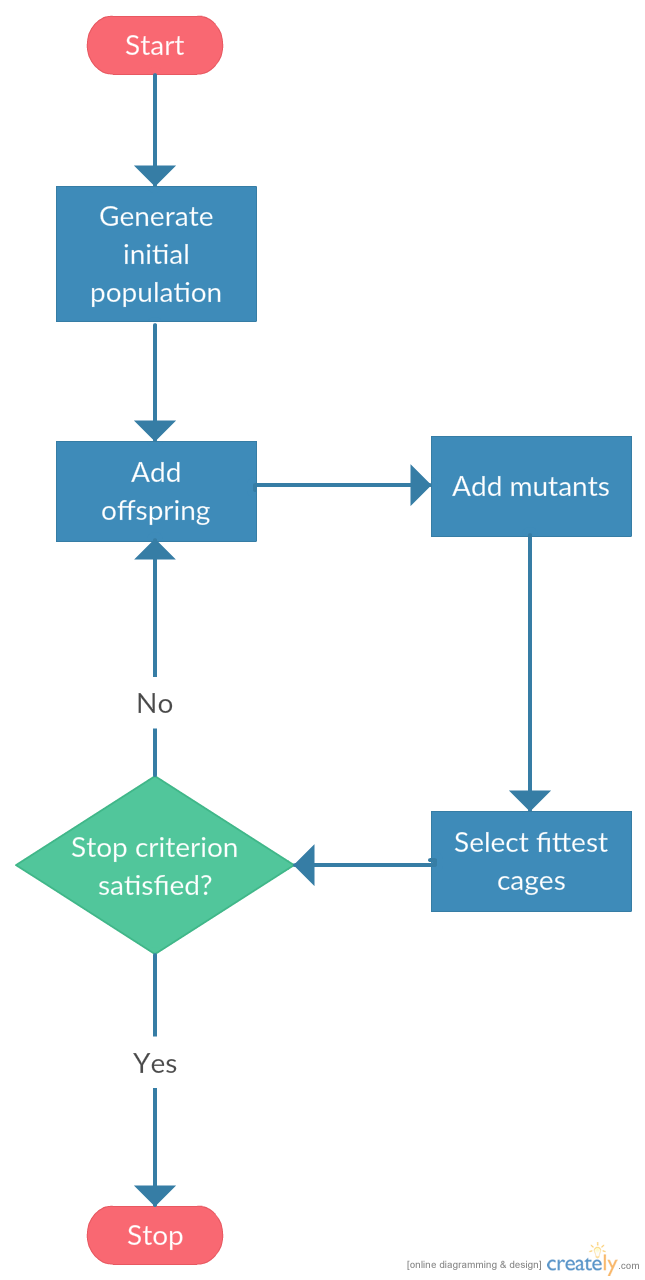
\includegraphics[scale=0.25]{./figures/program_overview/MMEA_flow.png}
	\caption{Flow diagram of MMEA execution.}
	\label{flow_diagram}
\end{figure}

\section{Design goals}

\section{Class overview}

\section{Style guide}

\section{Extending MMEA}

\end{document}